% This is LLNCS.DEM the demonstration file of
% the LaTeX macro package from Springer-Verlag
% for Lecture Notes in Computer Science,
% version 2.4 for LaTeX2e as of 16. April 2010
%
\documentclass[conference]{llncs}
%
\usepackage{url}
\usepackage{comment}
\usepackage{mathpartir}
\usepackage{listings}
\usepackage{alltt}
\usepackage{graphicx}
\usepackage{caption}
\usepackage{subfigure}
\usepackage{amssymb}
\usepackage{amsmath}
\usepackage{paralist, tabularx}
\usepackage{flushend}
\usepackage{multirow}
\usepackage{paralist}
\usepackage{algorithm}
\usepackage{algpseudocode}

\usepackage{pgfplots}
\pgfplotsset{width=11cm,height=8cm,compat=1.9}

\usepackage{mathtools}
\DeclarePairedDelimiter\ceil{\lceil}{\rceil}
\DeclarePairedDelimiter\floor{\lfloor}{\rfloor}


\usepackage[flushleft]{threeparttable}
\usepackage{footnote}

\makeatletter
\def\BState{\State\hskip-\ALG@thistlm}
\makeatother

\def\UrlBreaks{\do\/\do-}

\usepackage{color}
\definecolor{egmcolor}{rgb}{1.0,0.0,0.722}
\newcommand*{\egm}[1]%
%%
%% a)
{\textcolor{egmcolor}{\noindent\textbf{[egm:~}\textit{#1}]}}
%%
% Other things...
\newcommand{\figref}[1]{Figure~\ref{#1}}
\newcommand{\defref}[1]{Definition~\ref{#1}}
\newcommand{\tableref}[1]{Table~\ref{#1}}
\newcommand{\secref}[1]{Section~\ref{#1}}
\newcommand{\lemmaref}[1]{Lemma~\ref{#1}}
\newcommand{\cororef}[1]{Corollary~\ref{#1}}
\newcommand{\thmref}[1]{Theorem~\ref{#1}}
\newcommand{\algoref}[1]{Algorithm~\ref{#1}}

%\newtheorem{definition}{Definition}
%\newtheorem{theorem}{Theorem}
%\newtheorem{lemma}{Lemma}
%\newtheorem{corollary}{Corollary}

%
\begin{document}
\title{An Efficient Approach for Match Pair Approximation in Message Passing}

\author{Yu Huang \and Eric Mercer}
\institute{Brigham Young University \\
          \email{\{yuHuang,egm\}@byu.edu}}

\maketitle
%
%
\emergencystretch=1em


\begin{abstract} 
Asynchronous message passing paradigm is commonly used in high performance computing.
Message non-determinism makes the error detection in message passing programs very difficult. The prior work uses an over-approximation of the precise match pair records (each is a pair of a send and a receive that may potentially match in the runtime) to capture all possible message communication in a concurrent trace program (CTP). The SMT encoding with such a set of match pairs is able to detect errors including deadlock, message race, and zero-buffer incompatibility, however, is inefficient because of the exponential ways of match pair resolution.
This paper presents a new algorithm that under-approximates the match pairs iteratively: first matching a section in the CTP by queuing a fixed number of receives from a common process where the size depends on the user input, then distributing the same number of sends that may potentially match the receives from multiple processes to the section, and finally approximating the match pairs for the sends and receives in the section by comparing the ranking. The algorithm runs in quadratic complexity in the number of operations. Novel in the work is that the algorithm has the flexibility to generate different size of match pairs based on the user input. This paper further proves that the precise match pairs for any CTP can be generated with an appropriate input. The benchmarks show that all the errors are efficiently detected with a small set of match pairs generated by the new algorithm.
\end{abstract}

\keywords{Message Passing, MPI, SMT}

\newsavebox{\boxTZero}
\begin{lrbox}{\boxTZero}
\begin{minipage}[t]{0.4\linewidth}
\large
\begin{alltt}
00 \(r\sb{0}(\ast\ 0\ A\ w\sb{0})\)
01 \(w\sb{0}(r\sb{0})\)
02 \(r\sb{1}(\ast\ 0\ B\ w\sb{1})\)
03 \(w\sb{1}(r\sb{1})\)
04 \(r\sb{2}(1\ 0\ C\ w\sb{2})\)
05 \(w\sb{2}(r\sb{2})\)
06 \(s\sb{5}(0\ 1)\)
07 \(r\sb{3}(\ast\ 0\ D\ w\sb{3})\)
08 \(w\sb{3}(r\sb{3})\)
09 \(r\sb{4}(2\ 0\ E\ w\sb{4})\)
0A \(w\sb{4}(r\sb{4})\)


\end{alltt}
\end{minipage}
\end{lrbox}

\newsavebox{\boxTOne}
\begin{lrbox}{\boxTOne}
\begin{minipage}[t]{0.4\linewidth}
\large
\begin{alltt}
10 \(s\sb{0}(1\ 0)\)
11 \(s\sb{1}(1\ 0)\)
12 \(r\sb{5}(0\ 1\ F\ w\sb{5})\)
13 \(w\sb{5}(r\sb{5})\)
14 \(s\sb{2}(1\ 0)\)
\end{alltt}
\end{minipage}
\end{lrbox}

\newsavebox{\boxTTwo}
\begin{lrbox}{\boxTTwo}
\begin{minipage}[t]{0.4\linewidth}
\large
\begin{alltt}
20 \(s\sb{3}(2\ 0)\)
21 \(s\sb{4}(2\ 0)\)\end{alltt}
\end{minipage}
\end{lrbox}

% ---------------------------------------------------------------------
% END Save boxes
% ---------------------------------------------------------------------

\newcommand\examplefigone{
\begin{figure*}[tb]
\begin{center}
\setlength{\tabcolsep}{2pt}
\begin{tabular}[t]{c|c|c}
$\mathit{p_1}$ & $\mathit{p_2}$ & $\mathit{p_3}$ \\
\hline
\scalebox{0.8}{\usebox{\boxTZero}}&
\scalebox{0.8}{\usebox{\boxTOne}} &
\scalebox{0.8}{\usebox{\boxTTwo}}\\
\end{tabular}
\end{center}
\caption{A simple concurrent trace program.}
\label{fig:example}
\end{figure*}
}

 \section{Introduction}
%Asynchronous message passing is a prevalent programming model in high performance computing (HPC). The model consists of two operations, send and receive, that are essential to message communication. The message communication is complicated because of the non-determinism that a receive may be matched with more than one send in the runtime. The use of match pair, a pair of a send and a receive that may potentially match in the runtime, is able to capture the message communication.
%The semantics can also be complicated because of two buffering settings in the runtime, infinite buffer (messages are buffered in the system) and zero buffer (no buffering in the system). Further, typical message passing standard such as message passing interface (MPI) specifies a special communication that uses collective operations to synchronize a program leading to a more complex program behavior. 
%Given the semantics, several common problems exist in message passing applications: the user-provided assertion may be violated in an execution; the program may deadlock for unexpected matching of receives; and the program may be incompatible with zero buffer semantics, meaning that no feasible schedule exists under zero buffer setting. 
Asynchronous message passing is a prevalent programming model in high performance computing (HPC).
The idea of message passing is simple at the outset; processes communicate by sending messages from one to another. It does not take long, however, to realize that despite the simplicity of the programming model, there is a lot of subtlety in message passing that can impact program behavior. For example, depending on the library, a programmer must be aware of such things as message non-determinism (concurrent sends to a process can arrive in any order), buffering semantics in the runtime (a process may block if the buffer is full), or broad synchronization operations that message with  groups of processes at the same time (i.e., collective operations). This inherent complexity means that the problems of determining if a message passing program is free of deadlock, compatible with a given buffering semantics, or if the message non-determinism affects the correctness of the computation are all NP-complete \cite{DBLP:conf/kbse/HuangMM13,HuangNFM15}. Showing any of these properties for an input program is hard.

Prior work on program correctness in the message passing paradigm can be roughly grouped into dynamic analysis where an existing runtime is manipulated to explore different scheduling outcomes \cite{DBLP:conf/ppopp/VakkalankaSGK08,DBLP:conf/sbmf/SharmaGB12}, model checking where a model of the original program is analyzed \cite{DBLP:conf/vmcai/Siegel07,DBLP:conf/pvm/Siegel07}, runtime verification where the program execution is observed but not manipulated \cite{DBLP:conf/sc/VetterS00,DBLP:conf/parco/KrammerBMR03,DBLP:conf/ptw/HilbrichSSM09}, and symbolic model checking where a model of the program is symbolically analyzed with an SMT solver \cite{DBLP:conf/kbse/HuangMM13,HuangNFM15}. This paper looks specifically at symbolic model checking and ways to better leverage the SMT solver in witnessing program properties for message passing programs.

The most efficient types of encoding for symbolic model checking of message passing programs, where efficient means they scale to programs with a high degree of message non-determinism, rely on the concept of a \emph{match pair} and a \emph{concurrent trace program} abstraction (CTP) \cite{DBLP:conf/kbse/HuangMM13,HuangNFM15,DBLP:conf/fm/ForejtKNS14,DBLP:conf/atva/ElwakilYW10,DBLP:conf/issta/ElwakilY10}. 
A match pair is a send and receive pair that may be matched by the run-time in some feasible execution of the program \cite{DBLP:conf/kbse/HuangMM13,HuangNFM15,DBLP:conf/fm/ForejtKNS14,DBLP:conf/atva/ElwakilYW10,DBLP:conf/issta/ElwakilY10}. 
A CTP is an abstraction of the program that removes all branching so each process is a sequence of send, receive, and wait (e.g., a witness to the completion of a send or receive) operations \cite{DBLP:conf/kbse/HuangMM13,HuangNFM15}. 
The abstraction is constructed by observing the execution of the program in the run time for a given input. Symbolic model checking gives the SMT solver an encoded CTP with a set of match-pairs, and the solver then tries to select a subset of the given  match-pairs in such a way that the CTP deadlocks or violates an assertion. 

%The symbolic model checking requires a over-approximated set of match pairs as input. The set includes all the true match pairs and maybe a few match pairs that may never occur in the runtime. 
%The work then encodes the CTP into an SMT problem that uses a set of formulas to constrain the program behavior based on the semantics. The typical error such as deadlock, zero buffer incompatibility or assertion violation is then checked by solving the SMT problem. If a satisfying assignment exists for the SMT problem, then the error is detected where the match pairs are resolved to capture the message communication in a feasible program execution. If the SMT problem is unsatisfiable, the CTP is free of that error because no feasible schedule exists with any resolution of the match pairs. 

The size of the input match-pair set directly impacts the cost of the call to the SMT solver in the symbolic model checking of message passing programs; a large input set typically means an expensive solver call especially if there is a high-degree of message non-determinism. The idea in this paper is to reduce the cost of the solver call by reducing the size of the input match set to each call. Such a reduction cannot, however, be done naively; any match pair set must be \emph{message complete}.  A message complete match pair set for a CTP is one that lets the program run to completion (assuming it is free of deadlock). 

%As such, reducing the size of the input match pair set directly impacts the run time cost, typically, of the SMT solver. A straightforward idea to improve the performance, therefore, is to reduce the number of the match pairs. A naive way of reducing the match pairs such as randomly selecting a subset of the match pairs, however, is not sufficient. The input set of match pairs must be sufficient to complete the message communication in a program execution if the CTP is free of deadlock. A match pair set that has this property for a given CTP is termed \emph{message complete}.
%The input match pairs must satisfy two properties: program completion (the program can run to completion assuming no deadlocks exist) and message non-determinism (the set has a certain degree of non-determinism such that a receive may be associated with more than one match pairs).  
%The algorithm in this paper explores a way to generate such a reduced set of match pairs.

To reduce the number of match pairs and thereby decrease the cost of verification, this paper describes an iterative algorithm to successively generate under-approximations of the true set of match pairs until all match pairs are generated. The under-approximations retain the message complete property. 
Such an approach focuses on property witnessing rather than proofs of correctness as the intent is to witness program properties early in the iterations before the set of match pairs gets large.
%Since the correctness of a CTP can not be proved given an under-approximated set of match pairs, this paper only discusses the capability of error detection for the SMT encoding. 
%The primary goal is to improve bug finding in a CTP; although, since the algorithm is iterative, it is able to eventually produce a set of match pairs that includes all reachable match pairs in the CTP, therefore it proves correctness. 


Generally, the algorithm generates the match pairs in two steps. 
First, each process is sectioned, where a section contains a fixed number of sequential receives. The input number $k$ is used to roughly compute how many sends from each sender may potentially match the receives in a section, and therefore, determines the number of receives in this section. For each section, the algorithm precisely adds a set of sequences of sends from multiple potential sender processes. The sends in each sequence are distributed sequentially from the sender process. The total number of the sends added to the section is equal to the number of receives in the same section. 
%The number of the receives depends on three values that are statically known: the positive integer $k$ configured by the user, the number of all the potential sender processes and the number of the unmatched receives in the process. 
Match pairs for each section are then generated independently for the process. This independent sectioning effectively ignores combinations of match pairs, that are feasible, but only available when the considered concurrent outstanding sends are more than the number of receives in the section. 
Finally, the algorithm generates the match pairs for the sends and receives in the same section by a list of simple rules based on ranks \cite{DBLP:conf/kbse/HuangMM13}. A rank is a non-negative integer that represents the position of a send or a receive in a specific sequence in a section.


%The key insight of the solution is that each section is considered independently for match pair generation.  
%The algorithm does not generate the match pair for a send and a receive from two different sections, while in fact the send and the receive may match in the runtime. 
%As a result, the algorithm is able to under-approximate the precise match pairs as input to an SMT problem. 
%Due to the missed match pairs that are derived from matching sends and receives in different sections, the SMT problem may not encode the complete program behavior. However, if the problem is satisfiable, then it is known that a specific error exists for a feasible schedule that is resolved by the encoding. As such, the SMT encoding with a reduced set of match pairs can be used to detect errors. If the problem is, however, unsatisfiable for the under-approximated match pairs, it does not mean that there are provably no errors for any feasible execution in the runtime. It is then necessary to generate a larger set of match pairs by a new input K to capture more behavior for detection.


The paper includes the proof that the precise match pairs for any CTP can also be generated with a sufficiently large bound $k$. 
Experiments further show that the runtime cost of error detection is dramatically reduced as the errors are found with relatively small values of $k$ creating simple problem instances for the SMT solver. 
Experiments also show that the algorithm is able to scale to a program that employs a high degree of message non-determinism and/or a high degree of deep communication.
Deep communication in this context means that a process may receive many messages from each sender.
The contributions include,
\begin{compactitem}
\item the efficient algorithm that under-approximates the precise match pairs for a CTP, 
%where the size depends on a positive integer $k$ configured by the user,
\item the proof that the precise match pairs for any CTP can be generated by the new algorithm with an appropriate bound $k$, and
\item the results from the experiments using a set of benchmarks to demonstrate the improved ability of witnessing program properties.
\end{compactitem}

The rest of the paper is organized as follows: 
Sections 2 presents the definition and semantics of CTP; Section 3 presents the general algorithm in the paper; Section 4 gives the proof that the precise match pairs can be generated; Section 5 gives the experimental results; Section 6 discusses the related work; and Section 7 is the conclusion and future work.

\section{Concurrent Trace Program Definition and Semantics}

\examplefigone

This section explains message communication in a simple CTP consisting of a handful of operations. Consider the CTP in \figref{fig:example} that includes three processes that use non-blocking send ($s$) and non-blocking receive ($r$) for message communication. The nearest-enclosing wait ($w$) witnesses the completion of the receive \cite{DBLP:conf/kbse/HuangMM13}. The completion of any send or receive, is only confirmed when the send or the receive is matched in the runtime. Note that if the sender ID for a receive is ``$\ast$", then the receive is wildcard meaning that it may match a send from any sender. 
%The declarations of the local variables are omitted for space. The other operations related to computation are also omitted because they are not essential to the algorithm in the paper.

Picking up the scenario in \figref{fig:example}, process $p_1$ receives five messages from any sender or the specific senders and sends one message to $p_2$; process $p_2$ sends three messages to $p_1$ and receives a message from $p_1$; and process $p_3$ sends two messages to $p_1$. 


A set of match pairs represents a solution to the SMT problem if that set of match pairs is feasible. 
Feasible in this context means there exists a program trace allowed by the runtime that matches according to the solution set. In this example, a feasible program trace is equation (1). 
%Given the concurrency in the scenario, a feasible program trace is presented in equation (1).
\begin{equation}
%\scriptsize
\begin{split}
s_0\rightarrow r_0\rightarrow w_0\langle r_0\ s_0\rangle \rightarrow s_3\rightarrow r_1\rightarrow w_1\langle r_1\ s_3\rangle \rightarrow s_1\rightarrow r_2\rightarrow w_2\langle r_2\ s_1\rangle \\
\rightarrow s_5\rightarrow r_5\rightarrow w_5\langle r_5\ s_5\rangle \rightarrow s_4\rightarrow r_3\rightarrow w_3\langle r_3\ s_4\rangle \rightarrow s_2\rightarrow r_4\rightarrow w_4\langle r_4\ s_2\rangle
\end{split}
\end{equation} 
%In equation (1), the arrow ``$\rightarrow$" indicates the order of execution between two operations.
%The angle braces following a wait represents a match pair. For example, the match pair $\langle r_0\ s_0\rangle$ means that the send $s_0$ matches the receive $r_0$ at the wait $w_0$. 
As shown, the feasible trace in equation (1) implies a set of match pairs that represents a solution to the SMT problem from the prior work. The solution for equation (1) is $\{\langle r_0\ s_0\rangle, \langle r_1\ s_3\rangle, \langle r_2\ s_1\rangle, \langle r_5\ s_5\rangle, \langle r_3\ s_4\rangle, \langle r_4\ s_2\rangle\}$.


%Also, the sends and receives in equation (1) are totally ordered for completion. For example, the arrow between the match pair $\langle r_0\ s_0\rangle$ and the send $s_3$ shows that $r_0$ is matched before $s_3$ is matched in the runtime. 

Since the message matching is possibility non-deterministic in the presence of wildcard receives, there exist other feasible executions for the CTP in \figref{fig:example} where the receives are matched in different ways. For example,  the receive $r_0$ can be matched with the send $s_3$ instead of the send $s_0$ if $s_3$ arrives in $p_1$ earlier than $s_0$. As such, the message delivery for $r_0$ is non-deterministic and it is associated with two potential match pairs. 
Given the message non-determinism, the message communication can be resolved in many (and possibly exponential) ways. 
%Therefore, it is possible to capture all the message communication in a CTP only by adding all the potential match pairs in a single set. 
Therefore, to capture the behavior in other executions, new match pairs are needed.
For example, another feasible execution is presented in equation (2). As shown, the CTP in \figref{fig:example} deadlocks for this trace. 
\begin{equation}
%\scriptsize
s_0\rightarrow r_0\rightarrow w_0\langle r_0\ s_0\rangle \rightarrow s_1\rightarrow r_1\rightarrow w_1\langle r_1\ s_1\rangle \rightarrow s_3\rightarrow s_4 \rightarrow (\mathrm{Deadlock})
\end{equation} 
The deadlock occurs because there is no way to match the receives $r_2$ and $r_5$ after the sends $s_3$ and $s_4$ are issued. The use of the new match pair $\langle r_1\ s_1\rangle$ is essential to find the execution in equation (2) that makes the CTP in \figref{fig:example} deadlock.
The goal of the new algorithm in this paper is to generate a reduced set of the precise match pairs that can be used to finding such a trace with hidden errors.




%\section{Overview of SMT Encoding}

%define match pair in the format of SMT encoding

%discuss how match pairs are used in SMT encoding for error detection

The crucial idea behind the prior work is encoding a CTP into an SMT problem that uses a set of formulas to constrain the program behavior based on the semantics. 
The typical errors are then checked by solving the SMT problem with additional steps. If a satisfying assignment exists for the SMT problem, then the error is detected for a feasible schedule with a resolution of the match pairs to capture the message communication in the schedule. If the SMT problem is unsatisfiable, the CTP is free of that error because no feasible schedule exists with any resolution of the match pairs.

%In precise, the violation of assertions needs to encode the negation of the tested assertions into the SMT problem \cite{}; the zero buffer incompatibility requires more restricted formulas of the zero buffer semantics encoded in the SMT problem \cite{}; and the deadlock should launch a series of static analyses to first detect a potential deadlock before validating it with the SMT problem \cite{}.  

The SMT encoding relies on the \textit{happens-before} relation in \defref{def:hb}.
\begin{definition}
The happens-before relation, denoted as $\prec_{\mathtt{HB}}$, is a partial order over operations.
\label{def:hb}
\end{definition}
Given two operations, $A$ and $B$, if $A$ must complete before $B$ in a valid program execution, then $A \prec_{\mathtt{HB}} B$ will be an SMT constraint. 
The relation is derived from the program source and potential match pairs. 

The SMT encoding specifies the constraints from the program source such that the operations in each process has to be sequentially ordered. The happens-before relation is used to define a list of rules for the constraint of sequential order. Please refer to the prior work \cite{} for the full definition of these rules. 

The SMT encoding also needs to express the message communication in the given match pairs.
Informally, a match pair equates the shared components of a send and receive and constrains the send to happen before the nearest-enclosing wait of the receive. 

\begin{definition}
A match pair, $\langle r\ s\rangle$, for a receive $r$ and a send $s$ corresponds to the constraints:
\begin{compactenum}
\item $r$ and $s$ have a common destination;
\item $r$ and $s$ have a common source, or $r$ is a wildcard receive; and
\item $s \prec_{\mathtt{HB}} nw_r$, where $nw_r$ is the nearest-enclosing wait of $r$.
\end{compactenum}
\end{definition} 
If zero buffer semantics are applied, the \textit{happens-before} relation is further constrained for any match pair $\langle r\ s \rangle$ such that $s$ and $r$ are strictly ordered, meaning that there does not exist any operation $op$ such that $s \prec_{\mathtt{HB}} op$ and $op \prec_{\mathtt{HB}} r$. 

\begin{definition}
The match pair $\langle r\ s\rangle$ is precise if the receive $r$ is matched with the send $s$ in at least one feasible schedule.
\end{definition}

%\begin{corollary}
%The bogus match pair $\langle r\ s\rangle$ implies that the receive $r$ can not be matched with the send $s$ in any feasible schedule.
%\end{corollary}

The SMT problem in the prior work is given an over-approximated set of match pairs including all the precise match pairs and maybe some unprecise match pairs. Solving the problem needs to find one among all possible match pair resolutions that satisfies the constraints in the encoding. Consider the CTPs with large number of processes and high degree of message non-determinism, the number of match pair resolutions can be exponential. Therefore, the prior work does not scale for such a CTP. This paper presents a new approach that is able to generate a smaller set of match pairs, therefore, leading to a much more efficient SMT encoding.







\section{Main Algorithm}

%Notations: 
%Process set $P$
%receive list $R(p_{dest})$
%send list $S(p_{src}, p_{dest})$

%This section describes the general structure of the approach in this paper.
This section presents how to generate match pairs for each process in a CTP. 
Intuitively, the algorithm in \algoref{algo:main} sections each process, where each section contains a number of sequential receives. For each section, the algorithm distributes the same number of sends from multiple sender processes to match the receives in each section. Finally, the divided sections consisting of only sends and receives are input to the existing algorithm for match pair generation \cite{DBLP:conf/kbse/HuangMM13}. 

%a fixed number of sequential receives. It then distributes a sequence of sends from each sender process to match the receives in each section. The total number of sends is equal to the number of receives in each section. Finally, the algorithm generates the match pairs for the sends and the receives in the same section by simply comparing their ranks. The intuitive meaning of a rank is a non-negative integer that represents the position of a send or a receive in a specific sequence.

\begin{comment}
Sections = {}
cur = {}

while | R | \neq 0 {
  r = dequeue(R);
  S = ()
  if from(r) = * 
     Let S be such that \forall S' \in {S_i, S_j, ...} (count(S) \lte count(S’)) and | S | \neq 0)
	  count(S) += 1
  else
     Let S be such that S = Sender(r)

  cur = cur \cup {r, dequeue(S)}
  if \forall S \in {S_i, S_j, ...} (count(S) = k \vee |S| = 0 \vee | R | = 0)
     Sections  = Sections \cup {cur}
	  cur = {}
	  \forall S \in {S_i, S_j, ...} count(S) = 0;
}
\end{comment}


\begin{algorithm}
\caption{Main Entrance}\label{algo:main}
\begin{algorithmic}[1]
%\State $S\gets\emptyset$
\State $N_k\gets\Call{min}{|\mathit{sender}|\times k, |R|}$
\While{$|R|>0$}
\State $r \gets$ \Call{dequeue}{R}
\State $N_r\gets N_r+1$
\If{\Call{frm}{r}$=\ast$}
\State let $S$ be such that $\forall S^\prime \in \mathit{sender}(0<|S|\le |S^\prime| )$
\Else 
\State let $S$ be the sender of $r$
\EndIf
\State $s\gets$ \Call{dequeue}{$S$}
\If{$|S|=0$}
\State $\mathit{sender}\gets\mathit{sender} \setminus \{S\}$
\EndIf
%\State $S_i\gets S_i\cup\{s\}$ 
\State $\mathit{cur}\gets \mathit{cur}\cup \{r,s\}$
\If{$N_r=N_k$}
\State $\mathit{sections}\gets\mathit{sections}\cup\{\mathit{cur}\}$
\State $\mathit{cur}\gets\emptyset$
%\State $\forall S \in\{S_1,S_2,\ldots\}S\gets\emptyset$
\State $N_r\gets 0$
\State $N_k\gets\Call{min}{|\mathit{sender}|\times k, |R|}$
\EndIf
\EndWhile
\end{algorithmic}
\end{algorithm}



\begin{comment}

\begin{algorithm}
\caption{Main Entrance}\label{algo:main}
\begin{algorithmic}[1]
\For{$p_t\in \mathit{P}$}
%\State $N_{frm} \gets |frm_t|$
%\State $src(p)\gets\{p_1,p_2,\ldots,p_x\}$   \Comment{a set of all the potential sources for process $p$}
\While{$\mathit{NR}_{t}>0$}
\State $N_k\gets$\Call{SectionMatch}{$\mathit{k}$}
%$N_K \gets \Call{min}{|Src(p)|\times\mathit{K}, N_r(ALL,p)}$
\For{$p_f \in frm_t$}
\State $\mathit{NS_{tf}}\gets 0$
\EndFor
\State $\mathit{{NS}^\prime}\gets$\Call{DistributeSends}{$p_t$,$N_k$, $\mathit{NS}$}
\State $M\gets$\Call{MatchApprox}{$p_t$,$N_k$, $\mathit{{NS}^\prime}$}
\State \Call{remove}{$R_t$,$N_k$} 
%\State $R(p)\gets R(p)\setminus\{R(p)_i\mid 1\leq i\leq N_K\}$ 
\For{$p_{f^\prime} \in frm_t$} 
\If{$\mathit{NS}_{tf^\prime} > 0$}
\State \Call{remove}{$S_{tf^\prime}$,$\mathit{NS}_{tf^\prime}$}
\EndIf
%\State $S(p_i,p)\gets S(p_i,p)\setminus\{S(p_i,p)_j\mid 1\leq j\leq\mathit{n_s}(p_i,p)\}$
\EndFor
\EndWhile
\EndFor
\end{algorithmic}
\end{algorithm}

\end{comment}

\begin{comment}

\begin{algorithm}
\caption{Process Sectioning}\label{algo:main}
\begin{algorithmic}[1]
\For{$p_t\in \mathit{P}$}
\State let $R_t$ be the sequence of receives in $p_t$
\State let $S_t$ be the set of sequences of sends where each sequence contains the sends from a specific sender to $p_t$
\While{$|R_t|>0$}
\State $N_k\gets$\Call{SectionMatch}{$\mathit{k}$}
\State $(P_r,P_s)\gets$\Call{DistributeSends}{$R_t$,$S_t$,$N_k$}
\State $M\gets$\Call{MatchApprox}{$P_r$,$P_s$}
\EndWhile
\EndFor
\end{algorithmic}
\end{algorithm}

\begin{figure*}[tb]
\centering
\scalebox{0.8}{
\mprset{flushleft}
\begin{mathpar}
\inferrule[Deterministic Receive Command]
{
\mathit{frm}(r_0) = p_f \\ P_r = (r_a \ldots \bot) \\ P_r^\prime =  (r_0\ r_a\ \ldots \bot) \\
P_s(f) = (s_b\ \ldots\ \bot) \\ P_s^\prime = P_s[f\rightarrow(s_{f0}\ s_b\ \ldots\ \bot)] \\
N_k^\prime = N_k-1
}{
((r_0\ r_1\ \ldots\ \bot)\ ((0\rightarrow(s_0\ s_1\ \ldots\ \bot))\ \ldots (f\rightarrow(s_{f0}\ s_{f1}\ \ldots\ \bot))\ \ldots \bot)\ P_r\ P_s\ N_k)
\reduce{m} \\
((r_1\ \ldots\ \bot)\ ((0\rightarrow(s_0\ s_1\ \ldots\ \bot))\ \ldots (f\rightarrow(s_{f1}\ \ldots\ \bot))\ \ldots \bot)\ P_r^\prime\ P_s^\prime\ N_k^\prime)
}
\and
\inferrule[Wildcard Receive Command]
{
\mathit{frm}(r_0) = \ast \\ P_r = (r_a \ldots \bot) \\ P_r^\prime =  (r_0\ r_a\ \ldots \bot) \\
\forall f^\prime\in \mathit{frm}_t, P_s(f)\le P_s(f^\prime) \\ P_s(f) = (s_b\ \ldots\ \bot) \\ P_s^\prime = P_s[f\rightarrow(s_{f0}\ s_b\ \ldots\ \bot)] \\
N_k^\prime = N_k-1
}{
((r_0\ r_1\ \ldots\ \bot)\ ((0\rightarrow(s_0\ s_1\ \ldots\ \bot))\ \ldots (f\rightarrow(s_{f0}\ s_{f1}\ \ldots\ \bot))\ \ldots \bot)\ P_r\ P_s\ N_k)
\reduce{m} \\
((r_1\ \ldots\ \bot)\ ((0\rightarrow(s_0\ s_1\ \ldots\ \bot))\ \ldots (f\rightarrow(s_{f1}\ \ldots\ \bot))\ \ldots \bot)\ P_r^\prime\ P_s^\prime\ N_k^\prime)
}
\end{mathpar}
}
\caption{Machine reductions ($\reduce{m}$). }
\label{fig:machine}
\end{figure*}

\end{comment}


\subsection{Process Sectioning}

At a low level, the presentation needs to first explain a few data structures that are essential to the algorithm in \algoref{algo:main}.
$R$ is a list of all the sequential receives in a process.
$\mathit{sender}$ is a set of lists $\{S_i, S_j, \ldots\}$ that is the sends directed to the process grouped by the sending process.
$N_k$ is the number of receives in a single section.
$N_r$ is a number to count the receives added to the section and is initialized to $0$.
The set $\mathit{cur}$ is used to store the sends and receives in the current section. It is initialized to an empty set.
The set $\mathit{sections}$ is used to store all the sections.

Besides the data structures, the algorithm also applies a few auxiliary functions. 
$\Call{min}{a,b}$ returns one of the parameters that has a smaller value. 
$\Call{dequeue}{L}$ removes and returns the first element in the list $L$.
$\Call{frm}{r}$ returns the sender ID of the receive $r$.

Given the data structures and functions, \algoref{algo:main} works in several steps: 
\begin{compactenum}
\item Dequeuing the first receive $r$ from the list $R$ (line 3 to line 4);
\item Choosing a sender $S$ based on the sender ID of $r$ (line 5 to line 9);
\item Dequeuing the first send $s$ from the sender $S$ (line 10);
\item Removing the sender $S$ from $\mathit{sender}$ if there are no sends remained in $S$ (line 11 to line 13);
\item Adding the combination of $r$ and $s$ to the current section $\mathit{cur}$ (line 14);
\item Adding the current section $\mathit{cur}$ to the set $\mathit{sections}$ once $N_r$ is equal to $N_k$ (line 15 to line 20);
\item Repeating the above steps until $R$ is empty (line 2).
\end{compactenum}


$N_k$ is computed given two parameters: $|\mathit{sender}|\times\mathit{k}$ and $|R|$. The intuition is that the algorithm, if possible, distributes roughly average $k$ sends from each sender and therefore, adds $\mathit{sender}|\times\mathit{k}$ receives to a section. If there are not sufficient receives in $R$, then the algorithm adds all that remained in $R$ to the section, where the number is $|R|$. 

For each receive $r$, if the sender ID is $\ast$ indicating $r$ is wildcard, then the algorithm randomly chooses a sender $S$ that has the minimum count among all the senders at line 6. If $r$ is a deterministic receive, then $S$ is the specific sender for $r$ at line 8.

Given the steps above, the algorithm is able to section the process. If any section is matched at line 15, the variables $\mathit{cur}$, $N_r$ and $N_k$ need to be reset at line 17 to line 19. 

%Finally, the set $\mathit{sections}$ is input to the existing algorithm for match pair generation \cite{DBLP:conf/kbse/HuangMM13}, where the match pairs are generated independently for each section. 

 

\begin{comment}
$\mathit{P}$ is a set of all the processes in a CTP. 
$frm_t$ is a set of the unique identifiers of all the senders for the receiver $p_t$. 
The identifier of a sender can be removed from $frm_t$ once the sender has no send to be distributed to $p_t$.
The list $R_t$ contains all the sequential receives in process $p_t$.
%$\mathit{NR}_{tf}$ is the number of the receives in $R_t$ where they can only match the sends from process $p_f$. 
%The source can be ``$\ast$" indicating the wildcard receives.
%If the source is equal to ``$A$", then 
$\mathit{NR}_{t}$ is the number of all the receives in $R_t$.
The list $S_{tf}$ contains all the sequential sends from the sender $p_f$ to the receiver $p_t$. 
$\mathit{NS}_{tf}$ is the number of the sends in $S_{tf}$ that are distributed to a specific section.

Given the data structures defined, the presentation explains \algoref{algo:main} in detail.
The algorithm iteratively checks each receive at line 2 until $R_t$ is empty.  
$\mathrm{SECTIONMATCH}$ computes the number of receives in each section at line 3. The value is assigned to $N_k$. 
$\mathrm{DISTRIBUTESENDS}$ updates the count of the distributed sends ($\mathit{NS}$) from each sender to a common section in the receiver $p_t$ at line 7. 
$\mathit{NS_{tf}}$ is initialized for each sender $p_f$ at line 4 through line 6.
$\mathrm{MATCHAPPROX}$ then stores the generated match pairs for each section in $M$ at line 8. 
Finally, the receives and the sends in each section are removed from the CTP at line 9 through line 14. 
The function $\mathrm{REMOVE}$ removes elements from the beginning of a list given two inputs: the list to remove from and the number of operations to remove. 

\subsection{Section Match}

$\mathrm{SECTIONMATCH}$ is a simple equation in (3).
\begin{equation}
\Call{min}{|frm_t|\times\mathit{k}, \mathit{NR}_{t}}
\end{equation}
The function $\mathrm{MIN}$ returns the minimum among two numbers: $|frm_t|\times\mathit{k}$ and $\mathit{NR}_{t}$.
The first number indicates that the algorithm, if possible, distributes roughly average $k$  sends from each sender and therefore, adds $|frm_t|\times\mathit{k}$ receives to a section. If there are not sufficient receives in $R_t$, then the algorithm adds all that remained in $R_t$ to the section, where the number is $\mathit{NR}_{t}$.




\begin{lemma}
\label{lemma:section}
Each receive in a CTP is added to exactly one section by \algoref{algo:main}; each send in the CTP is also added to exactly one section if $\mathrm{DISTRIBUTESENDS}$ distributes the same number of sends to match the receives in any section.
\end{lemma}
\begin{proof}
\algoref{algo:main} initializes $N_k$ the number of the receives in a single section by $\mathrm{SECTIONMATCH}$, and removes these receives from $R_t$ immediately after executing $\mathrm{MATCHAPPROX}$ at line 8. It is assumed that the same number of potential sends are distributed to the section by $\mathrm{DISTRIBUTESENDS}$ and are removed from $S_{tf^\prime}$ for each potential sender $p_{f^\prime}$ at line 12. Therefore, a receive or a send can only be added once. 
Further, \algoref{algo:main} exhaustively matches sections for all the receives in any process $p_t$ until $\mathit{NR}_{t}$ is equal to zero. 
%Also, it is assumed that the number of sends is equal to the number of receives in a CTP. 
%Each section also contains equivalent receives and sends. 
Therefore, all the receives and sends in the CTP are partitioned into sections. 
$\Box$
\end{proof}
\lemmaref{lemma:section} is used to prove the key theorem later in the paper.

\end{comment}



%\section{Send Distribution}

\algoref{algo:distribute} implements a possible way of distributing the potential sends to a specific section by computing the count of sends ($n_s$) for the common destination $p$. The algorithm is part of the function $\mathrm{DISTRIBUTESENDS}$ in \algoref{algo:main}. $N$ is the count of sends that are waiting to be distributed and is initialized to $N_K$ at line 1.The algorithm then runs in two phases. The first phase (line 2 to line 11) updates $n_s$ according to the count of the deterministic receives (the receive that has a specific source). The second phase (line 12 to line 24) updates $n_s$ by averagely distributing the sends from each potential source in $Src(p)$ to the section until $N$ is equal to zero indicating that the send distribution is finished for the section. 

\begin{algorithm}
\caption{Distribute Sends}\label{algo:distribute}
\begin{algorithmic}[1]
\State $N\gets N_K$
\For{$i\gets 1$ to $N_K$}
%\If{$r$ is a deterministic receive}
\State let $p_{r}$ be the source of the receive $R(p)_i$
\If{$p_{r}\neq\ast$}
\State $\mathit{n_s}(p_{r},p)\gets \mathit{n_s}(p_{r},p)+1$
\State $N\gets N-1$   
\If{$\mathit{n_s}(p_{r},p) = N_s(p_{r},p)$}
\State $Src(p)\gets Src(p)\setminus\{p_{r}\}$
\EndIf
\EndIf
%\EndIf
\EndFor
%\State $\mathit{avg}\gets (N_{snder}>0) ? N_{rest} / {N_{snder}} : N_{rest}$
\While{$N>0$}
\State $\mathit{avg}\gets N / {|Src(p)|}$
\For{$p_{s}\in Src(p)$}
%\If{$\mathit{n_s}(src,dest) < N_s(src,dest)$}
\If{$\mathit{n_s}(p_{s},p)<\mathit{K}\vee (\forall p_{s}^\prime\in Src(p),\mathit{n_s}(p_{s},p)\leq\mathit{n_s}(p_{s}^\prime,p))$}
\State $N_s^+ = \Call{min}{avg,N_s(p_{s},p)-\mathit{n_s}(p_{s},p)}$
\State $\mathit{n_s}(p_{s},p)\gets\mathit{n_s}(p_{s},p)+N_s^+$
\State $N\gets N-N_s^+$
\If{$\mathit{n_s}(p_{s},p) = N_s(p_{s},p)$}
\State $Src(p)\gets Src(p)\setminus\{p_{s}\}$
\EndIf
\EndIf
%\EndIf
\EndFor
\EndWhile
\end{algorithmic}
\end{algorithm}

The first phase checks each receive $R(p)_i$ in the section at line 3. If the source $p_r$ of $R(p)_i$ is not equal to ``$\ast$" at line 4 indicating that $R(p)_i$ is a deterministic receive, $n_s(p_r,p)$ is then incremented by one at line 5 and $N$ is reduced by one at line 6. The intuition is that for any deterministic receive with the source $p_r$, there has to be at least one send from $p_r$ to be distributed for the receive. If $n_s(p_r,p)$ is equal to $N_s(p_r,p)$ at line 7 indicating that all the sends from $p_r$ to $p$ are distributed, then $p_r$ is removed from $Src(p)$ at line 8 indicating that $p_r$ cannot be considered as a potential source for the destination $p$. 

The second phase iteratively distributes the remaining $N$ sends from the potential sources in $Src(p)$ until $N$ is equal to zero at line 12. 
First, the variable $avg$ is assigned to a value that is calculated by dividing $N$ by the number of the potential sources ($|Src(p)|$) at line 13. 
Each potential source $p_{s}$ is then checked at line 14. 
The condition at line 15 specifies two cases for $p_{s}$ to distribute sends. The intuition is that each potential source has to distribute an approximately average number of the sends in the two cases. The first case indicates that $n_s(p_{s},p)$ is less than the average count $K$. The second case indicates that $p_{s}$ has the lower count of sends in $n_s$ than that of any other potential source in $Src(p)$. 
If the condition at line 15 is satisfied, the variable $N_s^+$ is assigned to the minimum of the two values: $avg$ and $N_s(p_{s},p)-\mathit{n_s}(p_{s},p)$. The value indicates that the $avg$ sends are distributed from $p_s$; or, if there are not enough sends, all the remaining sends from $p_{s}$ to $p$ are distributed.  
The distribution is enforced by incrementing the value of $n_s(p_{s},p)$ and reducing the value of $N$ at line 17 and line 18 respectively. Similar to the first phase, $p_{s}$ is removed from $Src(p)$ at line 20 if all the sends from $p_{s}$ to $p$ are distributed.  

\begin{lemma}
\algoref{algo:distribute} distributes $N_K$ sends from multiple sources to a single section for matching the same number of receives in the section.
\label{lemma:distribute}
\end{lemma}


%\subsection{Match Pair Approximation}

\algoref{algo:match} approximates the match pairs for the sends and receives in a specific section.
The algorithm is the part of the function $\mathrm{MATCHAPPROX}$ in \algoref{algo:main}. 
The match pair generation algorithm in the prior work \cite{DBLP:conf/kbse/HuangMM13} is directly applied to the sends and receives for a specific section. 
Intuitively, the algorithm checks all the pairs of receives and sends in the section, and prunes obvious matches that cannot exist in any runtime implementation of the specification by comparing ranks of sends and receives. 
A rank of a receive is its position in the receive list for the section. 
A rank of a send is its position in the send list from a particular sender to the section.    
Please refer to the prior work \cite{DBLP:conf/kbse/HuangMM13} for more detail of the algorithm. 


\algoref{algo:match} implies the ``match over-approximation" property in the prior work \cite{DBLP:conf/kbse/HuangMM13}. The paper presents this property in \lemmaref{lemma:match}. 

\begin{lemma}
\algoref{algo:match} over-approximates the match pairs for all the receives and sends in a specific section; that is saying, that all the precise match pairs (and maybe some unprecise match pairs) in the section are added to the output $M$.
\label{lemma:match}
\end{lemma}

%\begin{proof}
%\algoref{algo:match} must never claim to be able to prune the precise match pairs. The algorithm considers all the pairs for a send and a receive in a specific section. Also, the condition at line 4 only prunes the pairs that may never occur in the runtime: the first rule validates the endpoints consistent for the send and the receive; the second and third rules validate the FIFO order in message delivery according to the semantics. Therefore, only unprecise match pairs are pruned. $\Box$
%\end{proof}


%The condition at line 4 is then used to soundly prune the pair of $R(p)_i$ and $S(p_s,p)_j$ if they never match in the runtime with three rules. The first rule indicates that $R(p)_i$ is either a wildcard receive (the receive that may match a send from any source) or the source of $R(p)_i$ matches the source of $S(p_s,p)_j$. The second rule indicates that $i$ is greater or equal to $j$ meaning that the sends preceding $S(p_s,p)_j$ in $S(p_s,p)$ have to be matched with the receives in $p$. 
%\section{Algorithm}
\algoref{algo:main} describes the general structure of match pair generator in three steps: section match, sends distribution, and match pair approximation. 

$\mathit{P}$ is a set of processes. $Src(p)$ is a set of identifiers for the source processes that may distribute sends to match the receives on process $p$. A source process may be removed from $Src(p)$ if no send can be distributed from the process.
$R(p_{dest})$ is a list of all the receives in process $p_{dest}$. The order of the list is identical with that in the original program. $R(p_{dest})_j$ returns the $j$th. receive in the list.
The function $N_r(p_{src},p_{dest})$ returns the number of all the receives in $R(p_{dest})$ with the source $p_{src}$. If $p_{src}$ is equal to ``$ALL$", $N_r(ALL ,p_{dest})$ represents the number of all the receives in $R(p_{dest})$.
$S(p_{src},p_{dest})$ is a list of all the sends from the source $p_{src}$ to the destination $p_{dest}$. The order of the list is also identical with that in the original program. $S(p_{src},p_{dest})_i$ returns the $i$th. send in the list.
The function $N_s(p_{src},p_{dest})$ returns the number of all the sends in $S(p_{src},p_{dest})$. 

\begin{algorithm}
\caption{Main Entrance}\label{algo:main}
\begin{algorithmic}[1]
\For{$p\in \mathit{P}$}
\State $Src(p)\gets\{p_1,p_2,\ldots,p_x\}$   \Comment{a set of all the potential sources for process $p$}
\While{$N_r(ALL,p)>0$}
\State $N_K \gets \Call{min}{|Src(p)|\times\mathit{K}, N_r(ALL,p)}$
\For{$i\gets1$ to $x$}
\State $\mathit{n_s}(p_i,p)\gets 0$
\EndFor
\State $\mathit{n_s^\prime}\gets$\Call{DistributeSends}{$\mathit{n_s}$,$p$,$N_K$}
\State $M\gets$\Call{MatchApprox}{$\mathit{n_s^\prime}$,$p$,$N_K$}
\State \Call{remove}{$R(p)$,$N_K$} 
%\State $R(p)\gets R(p)\setminus\{R(p)_i\mid 1\leq i\leq N_K\}$ 
\For{$i\gets 1$ to $x$} 
\State \Call{remove}{$S(p_i,p)$,$n_s(p_i,p)$}
%\State $S(p_i,p)\gets S(p_i,p)\setminus\{S(p_i,p)_j\mid 1\leq j\leq\mathit{n_s}(p_i,p)\}$
\EndFor
\EndWhile
\EndFor
\end{algorithmic}
\end{algorithm}

The algorithm iterates over all the receives in each process $p$ until $N_r(ALL,p)$ is equal to zero at line 3 meaning that all the receives are removed from $R(p)$. 
The first step is ``section match" that matches multiple sections among the receives in $R(p)$ and all the sends in $S(p_{i},p)$ for any potential source $p_{i}\in Src(p)$ given an input $K$. 
The integer $\mathit{K}$ is used to compute the count of sends/receives ($N_K$) in each section at line 4. The function $\mathrm{MIN}$ returns the minimum of two values: $|Src(p)|\times\mathit{K}$ and $ N_r(ALL,p)$, indicating that each source in $Src(p)$ has $K$ sends in average to match the receives in $R(p)$ if possible, otherwise, the rest of the receives in $R(p)$ are all considered in the section. 

The function $\mathit{n_s}(p_{i},p)$ returns the count of sends from $p_i$ to $p$ in a specific section. The count is initialized to zero for each potential source $p_i$ at line 6 and is computed in the function $\mathrm{DISTRIBUTESENDS}$ given the input $n_s$, $p$ and $N_K$ at line 8. The new count $n_s^\prime$ is then used to approximate the match pairs for a specific section in the function $\mathrm{MATCHAPPROX}$ given two additional input $p$ and $N_K$.
The output $M$ stores the approximated match pairs. After that, the matched receives and sends in the section are removed from $R(p)$ and $S(p_i,p)$ at line 10 and line 12 respectively, indicating that they are not considered for match pair generation in the next section. The function $\mathrm{REMOVE}$ is used to remove a fixed number (the second input) of sends or receives from the beginning of a list (the first input). 
 

\begin{algorithm}
\caption{Distribute Sends}\label{algo:distribute}
\begin{algorithmic}[1]
\State $N\gets N_K$
\For{$i\gets 1$ to $N_K$}
%\If{$r$ is a deterministic receive}
\State let $p_{r}$ be the source of the receive $R(p)_i$
\If{$p_{r}\neq\ast$}
\State $\mathit{n_s}(p_{r},p)\gets \mathit{n_s}(p_{r},p)+1$
\State $N\gets N-1$   
\If{$\mathit{n_s}(p_{r},p) = N_s(p_{r},p)$}
\State $Src(p)\gets Src(p)\setminus\{p_{r}\}$
\EndIf
\EndIf
%\EndIf
\EndFor
%\State $\mathit{avg}\gets (N_{snder}>0) ? N_{rest} / {N_{snder}} : N_{rest}$
\While{$N>0$}
\State $\mathit{avg}\gets N / {|Src(p)|}$
\For{$p_{src}\in Src(p)$}
%\If{$\mathit{n_s}(src,dest) < N_s(src,dest)$}
\If{$\mathit{n_s}(p_{src},p)<\mathit{K}\vee (\forall p_{src}^\prime\in Src(p),\mathit{n_s}(p_{src},p)\leq\mathit{n_s}(p_{src}^\prime,p))$}
\State $N_s^+ = \Call{min}{avg,N_s(p_{src},p)-\mathit{n_s}(p_{src},p)}$
\State $\mathit{n_s}(p_{src},p)\gets\mathit{n_s}(p_{src},p)+N_s^+$
\State $N\gets N-N_s^+$
\If{$\mathit{n_s}(p_{src},p) = N_s(p_{src},p)$}
\State $Src(p)\gets Src(p)\setminus\{p_{src}\}$
\EndIf
\EndIf
%\EndIf
\EndFor
\EndWhile
\end{algorithmic}
\end{algorithm}


\algoref{algo:distribute} implements the function $\mathrm{DISTRIBUTESENDS}$ in \algoref{algo:main} that computes the count of sends ($n_s$) for the common destination $p$ in a specific section. $N$ is the count of sends that are not distributed and is initialized to $N_K$ at line 1.The algorithm then runs in two phases. The first phase (line 2 to line 11) updates $n_s$ based on the count of deterministic receives. The second phase (line 12 to line 24) updates $n_s$ by averagely distributing sends from any potential source in $Src(p)$ until $N$ is equal to zero. 

The first phase checks each receive in the section at line 2. If the source $p_r$ for the receive $R(p)_i$ is not equal to ``$\ast$" at line 4 meaning that $R(p)_i$ is a deterministic receive (the receive has a specific source), $n_s(p_r,p)$ is then incremented by one at line 5 and $N$ is reduced by one at line 6. The intuition is that for any deterministic receive with the source $p_r$, there has to be at least one send from $p_r$ to be distributed for the receive. If $n_s(p_r,p)$ is equal to $N_s(p_r,p)$ at line 7 indicating that all the sends from $p_r$ are distributed, then $p_r$ is removed from $Src(p)$ at line 8 indicating that it cannot be considered as a potential source for the destination $p$. 

The second phase iteratively distributes the remaining sends from any potential source in $Src(p)$ until $N$ is equal to zero at line 12. It first calculates the variable $avg$ by dividing $N$ by the number of potential sources ($|Src(p)|$) at line 13. It then checks each potential source $p_{src}$ at line 14. The condition at line 15 specifies two cases that allow $p_{src}$ to distribute sends. The intuition is that the two cases is able to distributes approximately average number of sends from each potential source. The first case indicates that $n_s(p_{src},p)$ is less than the average count $K$. The second case indicates that $p_{src}$ has lower count in $n_s$ than that of any other potential source in $Src(p)$. 
If the condition at line 15 is satisfied, the variable $N_s^+$ is assigned to the minimum of two values: $avg$ and $N_s(p_{src},p)-\mathit{n_s}(p_{src},p)$. The value indicates that the average number of sends are distributed if possible, otherwise, all the remaining sends from $p_{src}$ to $p$ are distributed.  
The distribution is enforced by incrementing $n_s(p_{src},p)$ and reducing $N$ at line 17 and line 18 respectively. Similar to the first phase, $p_{src}$ can be removed from $Src(p)$ at line 20 if all the sends from $p_{src}$ to $p$ are distributed.  


\begin{algorithm}
\caption{Match Approximate}\label{algo:match}
\begin{algorithmic}[1]
\For{$i\gets 1$ to $N_K$}
\State let $p_r$ be the source of the receive $R(p)_i$
\For{$j\gets 1$ to $\mathit{n_s}(p_s,p)$ for any possible sender $p_s$}
\If{$(p_r = \ast\vee p_r = p_s)\wedge i \geq j\wedge i \leq j + (N - \mathit{n_s}(p_s,p))$}
\State $M\gets M\cup\{\langle R(p)_i,S(p_s,p)_j \rangle\}$
\EndIf
\EndFor
\EndFor
\end{algorithmic}
\end{algorithm}

\algoref{algo:match} implements the function $\mathrm{MATCHAPPROX}$ in \algoref{algo:main} that approximates the match pairs for the receives in a common process $p$ in a specific section. The algorithm is inspired by the prior work \cite{} that uses ranks of sends and receives for match pair approximation. 

The algorithm first checks each receive with the rank from $1$ to $N_K$ in $R(p)$ at line 1. $i$ is the rank of the receive $R(p)_i$. 
For each receive, the algorithm checks each send with the rank from $1$ to $n_s(p_s,p)$ in $S(p_s,p)$ for each potential source $p_s$ at line 3.
$j$ is the rank of the send $S(p_s,p)_j$ that. The condition at line 4 then uses the same rule of rank comparison in \cite{} to soundly prune the pair $\langle R(p)_i,S(p_s,p)_j\rangle$ that may never occur in the runtime. Also, the condition checks that $R(p)_i$ is either a wildcard receive (the receive may match a send from any source) or the source of $R(p)_i$ matches the source of $S(p_s,p)_j$.
If the condition is satisfied, the pair is added to $M$ at line 5. 


%The condition at line 4 is then used to soundly prune the pair of $R(p)_i$ and $S(p_s,p)_j$ if they never match in the runtime with three rules. The first rule indicates that $R(p)_i$ is either a wildcard receive (the receive that may match a send from any source) or the source of $R(p)_i$ matches the source of $S(p_s,p)_j$. The second rule indicates that $i$ is greater or equal to $j$ meaning that the sends preceding $S(p_s,p)_j$ in $S(p_s,p)$ have to be matched with the receives in $p$. 






\input{Completeness}
\section{Experiments}
This section describes a series of experiments over a set of benchmarks to determine (1) the effectiveness of the algorithm is quickly witnessing properties of the input program, and (2) how well the algorithm controls the size of the match pair set as the bound $k$ increases.

The benchmark programs come from different sources. Three are derived from actual MPI programs and are used in other works for benchmarking \cite{benchmark:fevs,mpptest_benchmark,DBLP:conf/ppopp/XueLWGCZZV09}.

\begin{compactitem}
\item \textit{Diffu2DNoBa} is modified from the program \textit{Diffusion 2D}, which uses barriers to “partition” the message communication into several sections \cite{benchmark:fevs}. \textit{Diffu2DNoBa} removes the barriers from the original program so deadlocks are present in the new program. The program is also interesting because the messages to any receiver are distributed from a large set of senders.

\item \textit{Pktuse} is executed with only 5 processes -- each of which has a long sequence of messages to be sent to the other processes \cite{mpptest_benchmark}. The program uses wildcard receives only, therefore has a high degree of message non-determinism. 

\item \textit{Floyd} implements the shortest path algorithm for all the pairs of nodes \cite{DBLP:conf/ppopp/XueLWGCZZV09}. Each node communicates only with the immediate following neighbor. The program also has a large set of senders for each receiver. 
\end{compactitem}

The remaining four are synthetic programs created for this study.

\begin{compactitem}
\item \textit{DeepComm} is a simple program with one receiver and 4 senders. The program is designed to have a long sequence of sends for each sender.
This scenario issues only wildcard receives, so that the messages from different senders may race.

\item \textit{MultiM} is an extension to a program in the MCAPI library distribution \cite{DBLP:conf/kbse/HuangMM13}. The program adds extra iterations to the original program to generate longer execution trace. The program uses only wildcard receives and there is an interesting violation of assertion that only occurs in some possible executions.

\item \textit{Mismatch} is designed to contain a communication deadlock in execution. The program interleaves wildcard receives and deterministic receives in the program text. A deterministic receive may be orphaned in program execution leading to a deadlock as all the potential sends it need are matched with the preceding wildcard receives. 

\item \textit{MismatchEx} is an extension to the program in \figref{fig:example} that contains more sends and receives. Similar to the program in \figref{fig:example}, a deadlock may occur in deep execution. 
%No assertions are present in the program.
\end{compactitem}


These programs are tested for three types of properties: assertion violation, zero buffer compatibility and deadlock. 
The deadlock checking relies on a static pattern matcher to identify potential deadlock scenarios \cite{}. 
The experiments here use single pattern match, and the SMT encoding is to witness the feasibility of that match. The same pattern match is used for all experiments on any given deadlock example. 
The initial trace for any input program is generated by MPICH \cite{mpich}, a public implementation of the MPI standard.
The SMT encoding for each test is generated by the existing rules \cite{DBLP:conf/kbse/HuangMM13,HuangNFM15} and is solved by Z3 \cite{demoura:tacas08}. 
The experiments are run on a AMD A8 Quad Core processor with 6 GB of memory running Ubuntu 14.04 LTS. 
%A time limit of 2 hours is set for each test. The test aborts the verification process if it does not complete within the time limit.

\subsection{Effectiveness}

The \textit{effectiveness of property witnessing} are shown in \tableref{table:benchmarks} that divides the tests into three groups, where each group is the tests for a single type of property. Each group is labeled in the first column: ``AssertionV" means assertion violation; ``ZeroCom" means zero buffer compatibility; and ``DL" means deadlock. For each benchmark, $k$ is the minimum value at which the property is witnessed (if the property exists), or the value at which the over-approximated match set is generated (if the property does not exist). 
The column ``\#M" is the number of the generated match pairs for $k$. 
The column ``$\mathrm{Time}_k^\ast$" is the cumulative sum: $\sum_{i=1}^k\mathrm{Time}_i$, where $\mathrm{Time}_i$ is the runtime of checking satisfiability with the generated match pairs for $k=i$.
%The notation ``TO" means ``time out" (exceeding the time limit set for each test). 
The column ``Speed" reports the relative speedup over the running time of simply using the regular over-approximated match pair set: $\mathrm{Time}(Over-approximated) / \mathrm{Time}_k^\ast$.
%The symbol ``--" means that the $\mathrm{Speed}$ can not be computed because the test times out.

\begin{comment}

\begin{savenotes}
\begin{table*}[t]
\begin{center}
\scriptsize
\caption{Tests on Selected Benchmarks}\label{table:benchmarks}
     \begin{threeparttable}
     \def\arraystretch{1.5}
\begin{tabular}{c|c|c|c|p{0.25cm}|c|c|c|p{0.25cm}|c|c|c|c|c|c|c|}
		\cline{2-16}	  
& \multicolumn{3}{c|}{Test Programs} & \multicolumn{4}{c|}{Test 1} & \multicolumn{4}{c|}{Test 2} & \multicolumn{4}{c|}{Test 3}  \\ \cline{2-16}   
        & $Name$ & \#P & \#OP & $k$\tnote{w} & \#M & Time & Speed& $k$ & \#M & Time & Speed & $k$\tnote{+} & \#M & Time & Speed\\ \hline
         \multicolumn{1}{ |c|  }{\multirow{5}{*}{\rotatebox[origin=c]{90}{AssertV}}} 
          &  \textit{Diff2DNoBa} & 16 & 188 & 1\tnote{d} & 514 & 3.508s & 14.86 & 2\tnote{d}& 934 & 31.722s & 1.48 & 3\tnote{d}& 1,066 & 52.131s & 0.59 \\ \cline{2-16}
         \multicolumn{1}{ |c|  }{}&  \textit{DeepComm} & 5 & 180 & 1 & 240 & 0.837s & 1,647 & 5 & 960 & 10.547s & 131 & 15 & 2,760 & 1,379s & 1.00 \\ \cline{2-16}
\multicolumn{1}{ |c|  }{}&  \textit{Pktuse} &5 & 2048 &1 & 1,792 & 180s & $>$40 & 5   &    4,828      & 564s & $>$13 & 128 & 99,328 & TO & -- \\ \cline{2-16}
\multicolumn{1}{ |c|  }{}&  \textit{MultiM} & 3 & 266 & 1 & 500 & 10.892s & 295 & 5 & 1,300 & 24.397s & 132 & 100 & 20,300 & 3,218s & 1.00\\ \cline{2-16}
\multicolumn{1}{ |c|  }{}&  \textit{Floyd} &32 & 528 &1\tnote{d}& 1,928 & 29.925s & 0.97 & 2\tnote{d} &    1,928      & 30.621s & 0.48 & 3\tnote{d} & 1,928 & 29.043s & 0.32 \\ \hline
\hline
        
         \multicolumn{1}{ |c|  }{\multirow{7}{*}{\rotatebox[origin=c]{90}{ZeroCom}}} 
         &  \textit{Diff2DNoBa} & 16 & 188 & 1\tnote{d} & 514 & 1.749s & 3.07 & 2\tnote{d} & 934 & 3.053s & 1.12 & 3\tnote{d}& 1,066 & 5.375s & 0.53 \\ \cline{2-16}
        \multicolumn{1}{ |c|  }{} &  \textit{DeepComm} & 5 & 180 & 1 & 240 & 0.875s & 291 & 5 & 960 & 3.056s & 83 & 15 & 2,760 & 255s & 1.00 \\ \cline{2-16}
\multicolumn{1}{ |c|  }{}&  \textit{Pktuse} &5 & 2048 &1 & 1,792 & 121s & $>$59 & 5   &    4,828      & 449s & $>$16 & 128 & 99,328 & TO & -- \\ \cline{2-16}
\multicolumn{1}{ |c|  }{}&  \textit{MultiM} & 3 & 266 & 1 & 500 & 8.312s & 366 & 5 & 1,300 & 17.843s & 170 & 100 & 20,300 & 3,043s & 1.00\\ \cline{2-16}
\multicolumn{1}{ |c|  }{}&  \textit{Mismatch} &3 & 800 &1 & 204 & 2.904s & 3.06 & 30   &    622      & 3.297s & 2.69 & 50 & 793 & 8.872s & 1.00 \\ \cline{2-16}
\multicolumn{1}{ |c|  }{}&  \textit{MismatchEx} &3 & 296 &1 & 165 & 0.579s & 876  & 20   &    1,687      & 7.433s & 68 & 43 & 3,525 & 507s & 1.00  \\ \cline{2-16}
\multicolumn{1}{ |c|  }{}&  \textit{Floyd} &32 & 528 &1 & 1,928 & 89.032s & 1.02 & 5   &    1,928      & 90.908s & 1.00 & 10 & 1,928 & 91.155s & 1.00 \\ \hline
\hline

         \multicolumn{1}{ |c|  }{\multirow{3}{*}{\rotatebox[origin=c]{90}{DL}}} 
         &  \textit{Diff2DNoBa} & 16 & 188 & 1 & 514 & 3.479s & 13.50 & 2 & 934 & 44.060s & 1.07 & 3 & 1,066 & 46.974s & 1.00 \\ \cline{2-16}
\multicolumn{1}{ |c|  }{}&  \textit{Mismatch} &3 & 800 &1 & 204 & 2.160s & 6.61 & 30   &    622      & 10.061s & 1.42 & 50 & 793 & 14.286s & 1.00 \\ \cline{2-16}
\multicolumn{1}{ |c|  }{}&  \textit{MismatchEx} &3 & 296 &3 & 328 & 1.253s & 27.23 & 20   &    1,687      & 2.438s & 13.99 & 43 & 3,525 & 34.116s & 1.00 \\ \hline

       
\end{tabular}
\begin{tablenotes}
\item[w] $k$ is the minimum value with which the property is witnessed (if the property exists). 
\item[d] The property does not exist for the benchmark.
\item[+] The precise match pairs are over-approximated as $k$ is reached.
\end{tablenotes}
     \end{threeparttable}
\end{center}
\end{table*}
\end{savenotes}

\end{comment}

\begin{savenotes}
\begin{table*}[t]
\begin{center}
\scriptsize
\caption{Tests on Selected Benchmarks}\label{table:benchmarks}
     \begin{threeparttable}
    % \def\arraystretch{1.5}
\begin{tabular}{c|p{1.7cm}|c|c|c|c|c|c|}
		\cline{2-8}	  
& \multicolumn{3}{c|}{Test Programs} & \multicolumn{4}{c|}{Performance}   \\ \cline{2-8}   
        & $Name$ & \#P & \#Calls & $k$ & \#Match & Time & Speed\\ \hline
         \multicolumn{1}{ |c|  }{\multirow{5}{*}{\rotatebox[origin=c]{90}{AssertV}}} 
          &  \textit{Diff2DNoBa}\tnote{d} & 16 & 188 & 3 & 1,066 & 87.361s & 0.59 \\ \cline{2-8}
         \multicolumn{1}{ |c|  }{}&  \textit{DeepComm} & 5 & 180 & 1 & 240 & 0.837s & 1,647 \\ \cline{2-8}
\multicolumn{1}{ |c|  }{}&  \textit{Pktuse} &5 & 2048 &1 & 1,792 & 180s & $>$40 \\ \cline{2-8}
\multicolumn{1}{ |c|  }{}&  \textit{MultiM} & 3 & 266 & 1 & 500 & 10.892s & 295 \\ \cline{2-8}
\multicolumn{1}{ |c|  }{}&  \textit{Floyd}\tnote{d} &32 & 528 & 2 & 1,928 & 60.546s & 0.48 \\ \hline
\hline
        
         \multicolumn{1}{ |c|  }{\multirow{7}{*}{\rotatebox[origin=c]{90}{ZeroCom}}} 
         &  \textit{Diff2DNoBa}\tnote{d}& 16 & 188 & 3& 1,066 & 10.177s & 0.53 \\ \cline{2-8}
        \multicolumn{1}{ |c|  }{} &  \textit{DeepComm} & 5 & 180 & 1 & 240 & 0.875s & 291 \\ \cline{2-8}
\multicolumn{1}{ |c|  }{}&  \textit{Pktuse} &5 & 2048 &1 & 1,792 & 121s & $>$59 \\ \cline{2-8}
\multicolumn{1}{ |c|  }{}&  \textit{MultiM} & 3 & 266 & 1 & 500 & 8.312s & 366 \\ \cline{2-8}
\multicolumn{1}{ |c|  }{}&  \textit{Mismatch} &3 & 800 &1 & 204 & 2.904s & 3.06 \\ \cline{2-8}
\multicolumn{1}{ |c|  }{}&  \textit{MismatchEx} &3 & 296 &1 & 165 & 0.579s & 876  \\ \cline{2-8}
\multicolumn{1}{ |c|  }{}&  \textit{Floyd} &32 & 528 &1 & 1,928 & 89.032s & 1.02 \\ \hline
\hline

         \multicolumn{1}{ |c|  }{\multirow{3}{*}{\rotatebox[origin=c]{90}{DL}}} 
         &  \textit{Diff2DNoBa} & 16 & 188 & 1 & 514 & 3.479s & 13.50 \\ \cline{2-8}
\multicolumn{1}{ |c|  }{}&  \textit{Mismatch} &3 & 800 &1 & 204 & 2.160s & 6.61 \\ \cline{2-8}
\multicolumn{1}{ |c|  }{}&  \textit{MismatchEx} &3 & 296 &3 & 328 & 1.253s & 27.23  \\ \hline 
\end{tabular}
\begin{tablenotes}
\item[d] The property does not exist for the benchmark.
%\item[+] The precise match pairs are over-approximated as $k$ is reached.
\end{tablenotes}
     \end{threeparttable}
\end{center}
\end{table*}
\end{savenotes}



The results show that each property, if existing for the benchmark, is efficiently witnessed by the SMT encoding with the under-approximated match pairs in these benchmarks; it is not known if such early detection takes place in general. The tested properties for all the real programs can be witnessed with $k=1$. 
For example, the assertion violation for the program \textit{Pktuse} can be detected with $k=1$ where the speedup is greater than 40.

For the tests where the properties do not exist in the benchmarks, the results show slow down as expected, but the intent of this work is to improve the ability to find witnesses early rather than to prove correctness. 
For example, three tests are run for the program \textit{Diffu2DNoBa}, where $k$ is incremented from $1$ to $3$. 
The over-approximated match pairs are generated with $k=3$ that can be easily computed based on \thmref{theorem:precise}.


The tests for all the synthetic programs also show the properties can be witnessed with a potential for speed up, even if several tests are required to be run beforehand. For example, the program \textit{MismatchEx} is designed to contain a deadlock deep in an execution. The witness is found after $k$ is incremented to $3$, where the speed up is more than $27$ compared to the runtime with the over-approximated match set for $k=42$. The capability of witnessing properties with a low k-bound is especially helpful for the large programs to be feasible.

 
%also show that the runtime cost of the encoding is highly reduced with the match pairs generated with smaller $k$. For example, the assertion violation test for the program \textit{Diffu2DNoBa} takes 3 seconds to complete for $k=1$, while it takes to 67 seconds to solve the same encoding for $k=5$ only the match set is larger.

%To check zero buffer incompatibility, the precise match pairs are required because a zero buffer incompatible program indicates that all possible schedules are infeasible under zero buffer semantics. 
%As such, the zero buffer incompatibility for the program \textit{Diff2DNoBa} is only detected with $k=\infty$. 
%On the other hand, if any schedule for a program is able to run under zero buffer semantics, the program may never be zero buffer incompatible. As such, if a test shows that a zero buffer encoding is satisfiable for the program, then the program is proved to be zero buffer compatible. 
%The results show that the benchmarks excluding the program \textit{Diff2DNoBa} are zero buffer compatible by testing them with only a small set of match pairs.

%For deadlock detection, a prior static analysis is launched as preprocessing to find all the potential deadlocks in a program. If no potential deadlocks are found, then the SMT encoding is not required. For example, the deadlock test for the program \textit{MuitiM} is unavailable because no potential deadlock is detected.



\subsection{Scalability}
To evaluate how the input $k$ impacts the generated match pairs, the presentation discusses two benchmarks for how the sends are distributed from senders. The benchmarks are outside the set of programs discussed earlier and are defined based on the template program in \figref{fig:Texample}. The template program is simplified to contain only a receiver $p_r$ that issues a sequence of receives, and several senders $p_1,\ldots,p_m$ where each sender issues $N_s$ sends. Therefore, the number of receives in $p_r$ is $N_s\times m$.

\examplefigtemplate

\begin{figure}[!h]
\begin{minipage}{.5\textwidth}
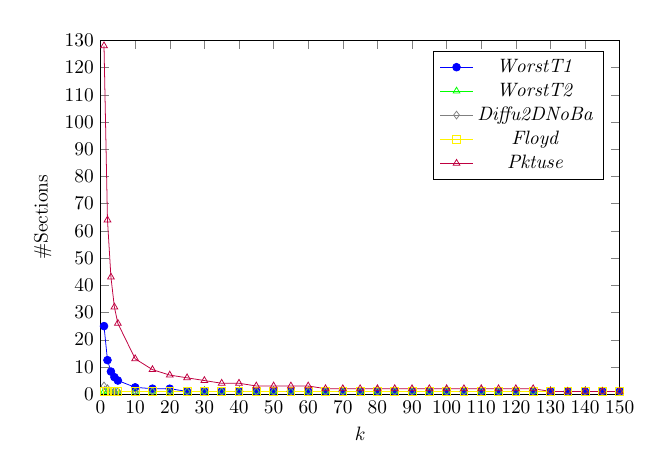
\begin{tikzpicture}[scale=0.7]
\begin{axis}[
    xlabel={$k$},
    ylabel={\#Sections},
    xmin=0, xmax=150,
    ymin=0, ymax=130,
    xtick={0,10,20,30,40,50,60,70,80,90,100,110,120,130,140,150},
    ytick={0,10,20,30,40,50,60,70,80,90,100,110,120,130},
    legend pos= north east,
    %ymajorgrids=true,
    grid style=dashed,
]
 
\addplot[
    color=blue,
    mark=*,
    ]
    coordinates {
    (1,25)(2,12.5)(3,8.3)(4,6.25)(5,5)(10,2.5)(15,2)(20,2)(25,1)(30,1)(35,1)(40,1)(45,1)(50,1)(55,1)(60,1)(65,1)(70,1)(75,1)(80,1)(85,1)(90,1)(95,1)(100,1)(105,1)(110,1)(115,1)(120,1)(125,1)(130,1)(135,1)(140,1)(145,1)(150,1)
    };

%\addplot[
  %  color=red,
   % mark=square,
   % ]
   % coordinates {
    %(1,25)(2,12.5)(3,8.3)(4,6.25)(5,5)(10,2.5)(15,2)(20,2)(25,1)(30,1)(35,1)(40,1)(45,1)(50,1)(55,1)(60,1)(65,1)(70,1)(75,1)(80,1)(85,1)(90,1)(95,1)(100,1)(105,1)(110,1)(115,1)(120,1)(125,1)(130,1)(135,1)(140,1)(145,1)(150,1)
   % };

\addplot[
    color=green,
    mark=triangle,
    ]
    coordinates {
    (1,1)(2,1)(3,1)(4,1)(5,1)(10,1)(15,1)(20,1)(25,1)(30,1)(35,1)(40,1)(45,1)(50,1)(55,1)(60,1)(65,1)(70,1)(75,1)(80,1)(85,1)(90,1)(95,1)(100,1)(105,1)(110,1)(115,1)(120,1)(125,1)(130,1)(135,1)(140,1)(145,1)(150,1)
    };
    
\addplot[
    color=gray,
    mark=diamond,
    ]
    coordinates {
    (1,3)(2,2)(3,1)(4,1)(5,1)(10,1)(15,1)(20,1)(25,1)(30,1)(35,1)(40,1)(45,1)(50,1)(55,1)(60,1)(65,1)(70,1)(75,1)(80,1)(85,1)(90,1)(95,1)(100,1)(105,1)(110,1)(115,1)(120,1)(125,1)(130,1)(135,1)(140,1)(145,1)(150,1)
    };
    
    \addplot[
    color=yellow,
    mark=square,
    ]
    coordinates {
    (1,1)(2,1)(3,1)(4,1)(5,1)(10,1)(15,1)(20,1)(25,1)(30,1)(35,1)(40,1)(45,1)(50,1)(55,1)(60,1)(65,1)(70,1)(75,1)(80,1)(85,1)(90,1)(95,1)(100,1)(105,1)(110,1)(115,1)(120,1)(125,1)(130,1)(135,1)(140,1)(145,1)(150,1)
    };
    
      \addplot[
    color=purple,
    mark=triangle,
    ]
    coordinates {
    (1,128)(2,64)(3,43)(4,32)(5,26)(10,13)(15,9)(20,7)(25,6)(30,5)(35,4)(40,4)(45,3)(50,3)(55,3)(60,3)(65,2)(70,2)(75,2)(80,2)(85,2)(90,2)(95,2)(100,2)(105,2)(110,2)(115,2)(120,2)(125,2)(130,1)(135,1)(140,1)(145,1)(150,1)
    };    
    
    \legend{\textit{WorstT1},\textit{WorstT2},\textit{Diffu2DNoBa},\textit{Floyd},\textit{Pktuse}}
 
\end{axis}
 
\end{tikzpicture}
\end{minipage}

\caption{The number of divided sections of varying the input $k$.}
\label{fig:relation:section}
\end{figure}

\begin{figure}[!h]
\begin{minipage}{.55\textwidth}
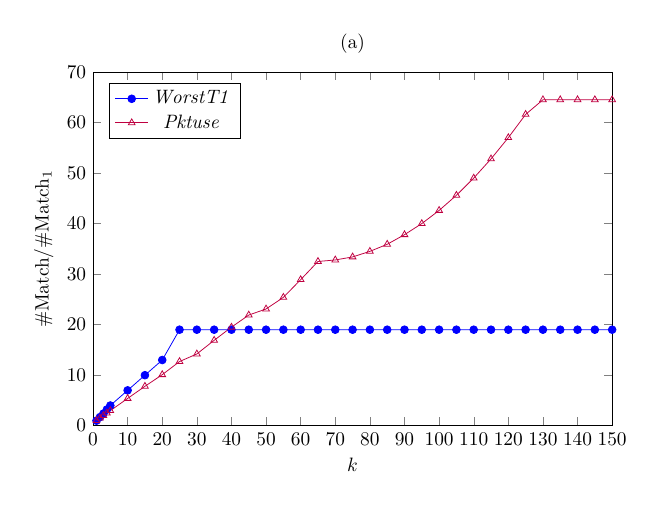
\begin{tikzpicture}[scale=0.7]
\begin{axis}[
   title = {(a)},
    xlabel={$k$},
    ylabel={\#Match$/$\#$\mathrm{Match}_1$},
    xmin=0, xmax=150,
    ymin=0, ymax=70,
    xtick={0,5,10,15},
    xtick={0,10,20,30,40,50,60,70,80,90,100,110,120,130,140,150},
    ytick={0,10,20,30,40,50,60,70},
    legend pos=  north west,
    %ymajorgrids=true,
    grid style=dashed,
]   

    
\addplot[
    color=blue,
    mark=*,
    ]
    coordinates {
    (1,1)(2,1.7)(3,2.4)(4,3.2)(5,4)(10,7)(15,10)(20,13)(25,19)(30,19)(35,19)(40,19)(45,19)(50,19)(55,19)(60,19)(65,19)(70,19)(75,19)(80,19)(85,19)(90,19)(95,19)(100,19)(105,19)(110,19)(115,19)(120,19)(125,19)(130,19)(135,19)(140,19)(145,19)(150,19)
    };
    

    
    \addplot[
    color=purple,
    mark=triangle,
    ]
    coordinates {
    (1,1)(2,1.5)(3,2)(4,2.5)(5,2.98)(10,5.4)(15,7.8)(20,10.1)(25,12.7)(30,14.2)(35,16.9)(40,19.5)(45,21.9)(50,23.1)(55,25.4)(60,28.9)(65,32.5)(70,32.8)(75,33.4)(80,34.5)(85,35.9)(90,37.8)(95,40)(100,42.6)(105,45.6)(110,49)(115,52.8)(120,57)(125,61.6)(130,64.5)(135,64.5)(140,64.5)(145,64.5)(150,64.5)
    };
    
    \legend{\textit{WorstT1},\textit{Pktuse}}
\end{axis}
\end{tikzpicture}
\end{minipage}

\begin{minipage}{.55\textwidth}
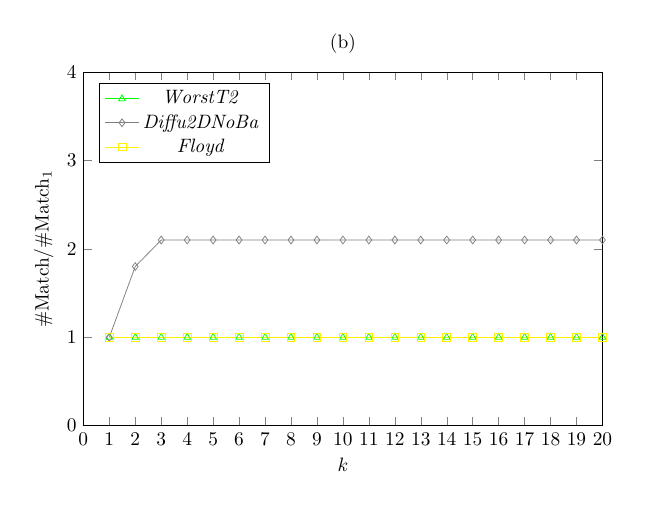
\begin{tikzpicture}[scale=0.7]
\begin{axis}[
   title = {(b)},
    xlabel={$k$},
    ylabel={\#Match$/$\#$\mathrm{Match}_1$},
    xmin=0, xmax=20,
    ymin=0, ymax=4,
    xtick={0,5,10,15},
    xtick={0,1,2,3,4,5,6,7,8,9,10,11,12,13,14,15,16,17,18,19,20},
    ytick={0,1,2,3,4},
    legend pos=  north west,
    %ymajorgrids=true,
    grid style=dashed,
]   
    
     %\addplot[
    %color=red,
   % mark=square,
    %]
    %coordinates {
%(1,1)(2,1)(3,1)(4,1)(5,1)(10,1)(15,1)(20,1)(25,1)(30,1)(35,1)(40,1)(45,1)(50,1)(55,1)(60,1)(65,1)(70,1)(75,1)(80,1)(85,1)(90,1)(95,1)(100,1)(105,1)(110,1)(115,1)(120,1)(125,1)(130,1)(135,1)(140,1)(145,1)(150,1)
 %   };
    
    \addplot[
    color=green,
    mark=triangle,
    ]
    coordinates {
    (1,1)(2,1)(3,1)(4,1)(5,1)(6,1)(7,1)(8,1)(9,1)(10,1)(11,1)(12,1)(13,1)(14,1)(15,1)(16,1)(17,1)(18,1)(19,1)(20,1)(25,1)(30,1)(35,1)(40,1)(45,1)(50,1)(55,1)(60,1)(65,1)(70,1)(75,1)(80,1)(85,1)(90,1)(95,1)(100,1)(105,1)(110,1)(115,1)(120,1)(125,1)(130,1)(135,1)(140,1)(145,1)(150,1)
    };
    
    \addplot[
    color=gray,
    mark=diamond,
    ]
    coordinates {
    (1,1)(2,1.8)(3,2.1)(4,2.1)(5,2.1)(6,2.1)(7,2.1)(8,2.1)(9,2.1)(10,2.1)(11,2.1)(12,2.1)(13,2.1)(14,2.1)(15,2.1)(16,2.1)(17,2.1)(18,2.1)(19,2.1)(20,2.1)(25,2.1)(30,2.1)(35,2.1)(40,2.1)(45,2.1)(50,2.1)(55,2.1)(60,2.1)(65,2.1)(70,2.1)(75,2.1)(80,2.1)(85,2.1)(90,2.1)(95,2.1)(100,2.1)(105,2.1)(110,2.1)(115,2.1)(120,2.1)(125,2.1)(130,2.1)(135,2.1)(140,2.1)(145,2.1)(150,2.1)
    };
    
    \addplot[
    color=yellow,
    mark=square,
    ]
    coordinates {
    (1,1)(2,1)(3,1)(4,1)(5,1)(6,1)(7,1)(8,1)(9,1)(10,1)(11,1)(12,1)(13,1)(14,1)(15,1)(16,1)(17,1)(18,1)(19,1)(20,1)(25,1)(30,1)(35,1)(40,1)(45,1)(50,1)(55,1)(60,1)(65,1)(70,1)(75,1)(80,1)(85,1)(90,1)(95,1)(100,1)(105,1)(110,1)(115,1)(120,1)(125,1)(130,1)(135,1)(140,1)(145,1)(150,1)
    };
    
    \legend{\textit{WorstT2},\textit{Diffu2DNoBa},\textit{Floyd}}
\end{axis}
\end{tikzpicture}
\end{minipage}

\caption{The relative growth of the number of match pairs of varying the input $k$, where $\mathrm{Match}_1$ is the number of the generated match pairs for $k=1$.}
\label{fig:relation:match}
\end{figure}

The first benchmark, \textit{WorstT1}, is constructed by restricting all the receives in \figref{fig:Texample} to be wildcard, which implies the worst case of message non-determinism. Also, let $m=4$ and $N_s = 25$ for the program so there are more than one sections divided for a set of possible $k$-bound. In contrast, the best case of message non-determinism is a program that only contains deterministic receives. As such, the matches for the best case are deterministic.
%In contrast, the second benchmark \textit{BestT1} is the best case of message non-determinism, where the program text is similar to \textit{WorstT1} only the receives are deterministic. 

The second benchmark, \textit{WorstT2}, is related to the worst case of wide communication. Wide communication in this context means that the sender only sends one message to the receiver. The program is constructed by setting $N_s=1$ and $m=100$. As for the best case of wide communication, the program has to contain only the deep communication where a receiver has exactly one sender. The presentation does not discuss this case as the matches are deterministic such that the messages are received in a fixed FIFO order. 

Given the two worst-case programs, the presentation discusses how the number of sections and the number of match pairs grow as $k$ increases for the two cases. 
The relationship between the number of sections and $k$ is illustrated in \figref{fig:relation:section}, and the relationship between the number of match pairs and $k$ is illustrated in \figref{fig:relation:match}.
Note that the values of y-axis in \figref{fig:relation:match} are computed by dividing the number of match pairs for any $k$ by the number of match pairs for $k=1$.

\figref{fig:relation:section} shows that the growth of the number of sections is not linear for the program \textit{WorstT1}. As such, incrementing $k$ may not be meaningful if the number of sections does not change. The algorithm only outputs the generated match pairs to the SMT encoding if the number of sections has changed.
Since the number of the generated match pairs per section is also non-linear according to the complexity of $\mathrm{MatchApprox}$ in \algoref{algo:main}, the total number of the match pairs for \textit{WorstT1} in \figref{fig:relation:match} (a) has a sharp growth between small values of $k$, and then grows more gently until it reaches the limit, which represents the over-approximated match pairs. This observation demonstrates that the algorithm scales for a small range of $k$ where the generated match set is small.

%The program \textit{BestT1} has the same growth of the number of sections with that for \textit{WorstT1} (not shown in \figref{fig:relation} (a)) because the send distribution has no difference between the two programs. 
%Since all the receives are deterministic in the program \textit{BestT1} indicating the matches are also deterministic, the number of the match pairs in \figref{fig:relation} (b) does not grow across $k$.

For the program \textit{WorstT2}, \figref{fig:relation:section} shows that the number of sections is always one as expected because only one section can be divided for wide communication. 
As such, the total number of match pairs for \textit{WorstT2} in \figref{fig:relation:match} (b) does not change. 

Based on the discussion of message non-determinism and wide communication, the synthetic programs discussed earlier can be grouped. The programs \textit{DeepComm} and \textit{MultiM} are close to the worst case of message non-determinism as only wildcard receives are employed in both programs. For the wide communication, no synthetic program is close to the worst case. Instead, all the programs show a certain degree of deep communication. 

The real programs can also be classified for message non-determinism and wide communication. \figref{fig:relation:section} and \figref{fig:relation:match} further plot the relations for the real programs. 
The programs \textit{Diff2DNoBa} and \textit{Floyd} uses more wide communication, therefore, their growths in \figref{fig:relation:match} rapidly reach the bound of match pairs. In contrast, the program \textit{Pktuse} employs a large degree of deep communication with many wildcard receives. As such, \textit{Pktuse} in \figref{fig:relation:match} (a) gradually grows to the bound as $k$ increases to $128$.
Thefore, the presentation demonstrates that the algorithm is able to scale to a program with a high degree of message non-determinism and a high degree of deep communication.



\section{Related Works}
There are several works related to match pairs.
Sharma et al. proposed the first push button model checker for MCAPI -- MCC \cite{DBLP:conf/fmcad/SharmaGMH09}. It indirectly controls the MCAPI runtime to verify MCAPI programs under zero buffer semantics. An obvious drawback of the work is its inability to analyze infinite buffer semantics which is known as a common runtime environment in message passing. A key insight, though, is the direct use of match pairs -- couplings for potential sends and receives.

A precise SMT encoding technique is proposed for detecting user-provided assertions for MCAPI programs \cite{DBLP:conf/kbse/HuangMM13}. The encoding is sound and complete and is easy to use to reason about infinite buffer semantics without requiring a precise match set. The work also provides an algorithm that runs in quadratic time complexity to generate a over-approximated match set based on the given execution trace. This approach is extended to checking zero buffer incompatibility for MPI semantics \cite{HuangNFM15}. 

A hybrid approach of static analysis and dynamic analysis also uses the SMT technique for detecting deadlocks in the pattern of orphaned receive \cite{HuangDeadlock}. This approach first detects all possible potential deadlocks statically, then prunes the infeasible deadlocks by an abstracting machine with counting, and finally validate the deadlock for a feasible schedule. The validation require the SMT encoding for orphaned receive deadlock. 

Forejt et al. proposed a SAT based approach to detect deadlock in a single-path MPI program \cite{DBLP:conf/fm/ForejtKNS14}. The solution is correct and efficient for programs with a low degree of message non-determinism. However, since the size of the encoding is cubic, checking large programs is time consuming. The work also requires a match pair set.

There are other solutions for message passing program analysis.
The dynamic analyzer ISP implements the POE algorithm, a Dynamic Partial Order Reduction (DPOR) algorithm \cite{DBLP:conf/popl/FlanaganG05} applied to MPI programs \cite{DBLP:conf/ppopp/VakkalankaSGK08}. 
An extension is the MSPOE algorithm \cite{DBLP:conf/sbmf/SharmaGB12}. It operates by postponing the cooperative operations for message passing in transit until each process reaches a blocking call. It then determines the potential matches of send and receive operations in the runtime. The solution is able to detect errors such as assertion violation and deadlock in an MPI program.
A drawback of ISP is that it does not scale for large programs due to state explosion.

Umpire is an approach of runtime verification for checking multiple MPI errors such as deadlock and resource tracking \cite{DBLP:conf/sc/VetterS00}. The error checking is taken by spawning one manger thread and several outfielder threads in the execution of an MPI program. A drawback of the approach is that it relies on a concrete execution, which may miss the errors in the other execution trace.
An extension to Umpire is Marmot \cite{DBLP:conf/parco/KrammerBMR03}. The work uses a centralized sever instead of multiple threads for error checking. Another extension to Umpire is MUST \cite{DBLP:conf/ptw/HilbrichSSM09}. The structure of MUST allows the users to execute the error checking either in an application process itself or in extra processes that are used to offload these analyses. 
However, just like Umpire and Marmot, the approach is neither sound nor complete for deadlock detection. 

MPI-Spin is integrated in the model checker SPIN \cite{DBLP:journals/tse/Holzmann97}, for verifying MPI programs \cite{DBLP:conf/vmcai/Siegel07,DBLP:conf/pvm/Siegel07}. It generates a model of an MPI program and symbolically executes it. It does not scale to large programs with a large degree of message non-determinism.

Vo et al. used Lamport clocks to update the auxiliary information via piggyback messages \cite{DBLP:conf/sc/VoAGSSB10,DBLP:conf/IEEEpact/VoGKSSB11}. While completeness is abandoned in their analysis, they show the work is useful and efficient in practice. 


%Elwakil et al. also used SMT techniques to reason about the program behavior in the MCAPI domain \cite{DBLP:conf/issta/ElwakilY10,DBLP:conf/atva/ElwakilYW10}. State-based and order-based encoding techniques are both used. These techniques fail to reason about the infinite buffer semantics and require a precise match set which is non-trivial to compute beforehand.


\section{Conclusion and Future Work}
This paper presents a new algorithm that generates the match pairs for message passing programs in the context of a CTP.
First, the algorithm sections each process where each section contains roughly $k$ sends from each sender that may match the same number of receives in the section. The bound $k$ is a user input.
The algorithm then approximates the match pairs by comparing the ranks for all the sends and receives in each section \cite{DBLP:conf/kbse/HuangMM13}. The key insight of the algorithm in this paper is that the match pairs for each section are generated independently. 
A send and a receive from two different sections can not be considered for matching. 
This paper also proves that all the precise match pairs for a CTP can be generated with the \textit{max bound} of $k$. Experiments demonstrate that all the properties in the benchmarks can be efficiently witnessed with under-approximated match pairs generated by the new algorithm. Experiments also show that the algorithm is able to scale to a program that employs a high degree of message non-determinism and/or a high degree of deep communication.

A restriction of the new algorithm is that it is incapable of approximating the match pairs for sends and receives from branches. Future work will explore new approach to handle branches.




\bibliographystyle{splncs03}
\bibliography{bib/paper}
\end{document}
